%% paper/sections/08_mechanism_analysis.tex
%% §8 Mechanism Analysis — 5 분류군별 fail/success 메커니즘 분석

\section{메커니즘 분석}
\label{sec:mechanism}

본 절은 \S\ref{sec:results}의 측정 결과에서 발견된 패턴들의 메커니즘을 분석한다.
각 분류군의 실패 또는 성공 원인을 정리하고, \algname 의 design 결정을 그 메커니즘으로 정당화한다.

%% figures/fig6_class_taxonomy.tex
%% Fig.6 — 5 분류군 dendrogram (단일 컬럼 fit)

\begin{figure}[t]
\centering
\resizebox{0.95\columnwidth}{!}{%
\begin{tikzpicture}[
    x=0.85cm, y=0.65cm,
    root/.style={rectangle, draw, rounded corners=2pt, thick, fill=blue!18,
                 font=\scriptsize\bfseries, align=center,
                 minimum width=3.5cm, minimum height=0.6cm},
    class/.style={rectangle, draw, rounded corners=1pt, fill=yellow!15,
                  font=\tiny\bfseries, align=center,
                  minimum width=1.3cm, minimum height=0.85cm,
                  inner sep=1pt},
    rep/.style={font=\tiny, align=center, inner sep=1pt},
    pos/.style={text=green!50!black, font=\tiny\bfseries},
    neg/.style={text=red!60!black, font=\tiny},
]
% Root
\node[root] (root) at (0, 3.2) {CPU resource utilization (24 candidates)};

% 5 classes
\node[class] (A) at (-4, 1.8) {A\\Direct\\kernel};
\node[class] (B) at (-2, 1.8) {B\\System\\isolation};
\node[class] (C) at (0,  1.8) {C\\Sub-step\\sched.};
\node[class] (D) at (2,  1.8) {D\\Aux.\\workload};
\node[class] (E) at (4,  1.8) {E\\Concurrent\\aux.};

% Lines root-to-class
\foreach \child in {A, B, C, D, E} {
    \draw[thick, gray!60] (root.south) -- (\child.north);
}

% Representatives
\node[rep, neg] at (-4, 0.7) {AMX matmul};
\node[rep, neg] at (-4, 0.3) {Jacobi (-94\%)};
\node[rep, pos] at (-2, 0.7) {NUMA pin};
\node[rep, neg] at (-2, 0.3) {4-OS stack};
\node[rep, neg] at (0,  0.7) {task-pool};
\node[rep, neg] at (0,  0.3) {(catastrophic)};
\node[rep, neg] at (2,  0.7) {AMX draft};
\node[rep, neg] at (2,  0.3) {cold-KV};
\node[rep, pos] at (4,  0.7) {\textbf{branchy 100\,ms}};
\node[rep      ] at (4,  0.3) {regular};

% Class to rep
\foreach \c/\y in {A/0.3, B/0.3, C/0.3, D/0.3, E/0.3} {
    \draw[gray!40, thin] (\c.south) -- ($(\c.south)+(0,-0.3)$);
}

% Legend
\node[font=\tiny, anchor=west, text=green!50!black] at (-4.5, -0.4) {green = positive};
\node[font=\tiny, anchor=west, text=red!60!black]   at (-0.5, -0.4) {red = negative};
\end{tikzpicture}%
}
\caption{5 분류군 taxonomy. 분류군 B 의 NUMA pin 과 분류군 E 의 branchy auxiliary 만 양성, 나머지는 분류군별 공통 메커니즘으로 실패.}
\label{fig:class-taxonomy}
\end{figure}


\subsection{분류군 A 실패 메커니즘: H2D/D2H 동기화 비용 누적}

분류군 A(직접 CPU 커널 대체)의 7개 기법이 모두 e2e 처리량 증가에 실패한 근본 원인은 \emph{critical path 안에 H2D/D2H 동기화가 추가}되기 때문이다.
microbench 수준에서 AMX BF16 matmul은 GPU H100 FP8 대비 약 3배 빠르지만, 다음의 비용이 추가된다.

\begin{itemize}
  \item H2D PCIe transfer: $\sim$1\,ms (텐서 크기 의존)
  \item CPU 커널 실행: $\sim$3\,ms (microbench 1.5--5$\times$ speedup의 결과)
  \item D2H PCIe transfer: $\sim$1\,ms
  \item CUDA stream 동기화: $\sim$0.5\,ms (launch overhead)
\end{itemize}

총 $\sim$5.5\,ms의 추가 비용이 step 주기 $\tgpu \approx 40$\,ms의 약 14\,\%를 점유하므로, microbench 이득이 sync overhead로 상쇄된다.
``4-method Jacobi router''의 $-94.2\,\%$ catastrophic 결과는 LM-head 행렬 곱이 1{,}810\,ms로 너무 무거워 165개 chat 요청에 대해 큐가 직렬화된 극단적 사례이다.

이 분석은 \algname 의 Stage 2(\textsc{Chord})에서 분류군 A를 lever pool에서 제외하는 design 결정을 정당화한다.

\subsection{분류군 B 부분 성공 메커니즘: NUMA 비대칭의 hardware-level 활용}

분류군 B(시스템 격리) 중 NUMA 고정 단독 기법만 multi-run binding을 통과한다(Table~\ref{tbl:multirun}).
이는 NUMA distance 비대칭(local 10 vs. remote 21)이 \emph{hardware-level 의 일관된 효과}를 갖기 때문이다.

vLLM의 텐서 병렬 인스턴스는 NCCL all-reduce 트래픽이 매우 빈번하므로, 인스턴스의 CPU/메모리 affinity를 GPU PCIe affinity가 있는 NUMA 노드와 일치시키면 cross-socket QPI 트래픽이 제거된다.
이는 측정마다 일관된 latency 회복을 보장하며, 따라서 1-run noise floor에 의존하지 않는 robust 양성 신호를 만든다.

반면 cgroup/hugepages/taskset 같은 OS-level 단독 isolation은 vLLM의 Python 프로세스가 이미 page-fault rate가 낮은 환경에서는 marginal effect만 보인다.
또한 이들을 여러 개 stacking 하면 context-switch와 cache eviction이 누적되어 destructive interference를 발생시킨다(Table~\ref{tbl:superposition}의 4-OS-lever residual $-1.18$\,pp).

이 분석은 Theorem~\ref{thm:superposition}의 \emph{same-domain interference cost} $\varepsilon_{\text{same}} \approx 1.18$\,pp의 직접적 메커니즘 설명이다.

\subsection{분류군 C 실패 메커니즘: task-pool lock contention}

분류군 C(sub-step CPU 스케줄링)는 GPU step 내부의 attention/linear sub-phase 경계에 CPU 작업을 burst하는 접근이다.
이는 이론적으로 GPU의 sub-phase idle window를 활용할 수 있어 매력적이지만, 본 측정에서 task-pool 기반 구현은 catastrophic failure를 보였다.

근본 원인은 \emph{task-pool의 enqueue/dequeue lock 경쟁이 step 내부 critical path를 stall} 시키기 때문이다.
spec-decode backend의 step latency는 약 35--44\,ms로 매우 짧고, 이 시간 안에서 sub-phase 신호 IPC(p50 $\sim$4.82\,us)는 OK이지만 task-pool lock acquisition은 contention 시 수 ms까지 spike한다.
이로 인해 spec-decode backend에서 $-14$\,\%부터 $-20$\,\%의 catastrophic 결과가 발생한다.

이 분석은 \algname 이 sub-step 스케줄링 대신 \emph{step boundary 외부의 별도 process}로 보조 작업을 분리하는 design 결정의 메커니즘 근거이다.

\subsection{분류군 E 성공 메커니즘 (역설): 정렬 + prefetcher 억제}

%% figures/fig3_pattern_cycle_grid.tex
%% Fig.3 — 2×3 work pattern × cycle ablation heatmap (단일 컬럼 fit)

\begin{figure}[t]
\centering
\resizebox{0.90\columnwidth}{!}{%
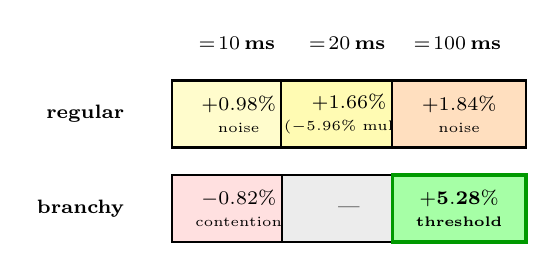
\begin{tikzpicture}[
    x=1.4cm, y=1.0cm,
    cell/.style={rectangle, draw, minimum width=1.7cm, minimum height=0.85cm,
                 align=center, font=\scriptsize, thick, inner sep=1pt},
    header/.style={font=\scriptsize\bfseries, align=center},
    rowlabel/.style={font=\scriptsize\bfseries, align=center, anchor=east},
]
% Column headers
\node[header] at (0, 1.5)  {$\tcpu\!=\!10$\,ms};
\node[header] at (1.0, 1.5) {$\tcpu\!=\!20$\,ms};
\node[header] at (2.0, 1.5) {$\tcpu\!=\!100$\,ms};

% Row labels
\node[rowlabel] at (-0.95, 0.6) {regular};
\node[rowlabel] at (-0.95, -0.6) {branchy};

% Regular row
\node[cell, fill=yellow!20] at (0, 0.6)
    {$+0.98\%$\\\tiny noise};
\node[cell, fill=yellow!30] at (1.0, 0.6)
    {$+1.66\%$\\\tiny ($-5.96\%$ multi)};
\node[cell, fill=orange!25] at (2.0, 0.6)
    {$+1.84\%$\\\tiny noise};

% Branchy row
\node[cell, fill=red!12] at (0, -0.6)
    {$-0.82\%$\\\tiny contention};
\node[cell, fill=gray!15] at (1.0, -0.6) {---};
\node[cell, fill=green!35, very thick, draw=green!60!black] at (2.0, -0.6)
    {$\mathbf{+5.28\%}$\\\tiny\textbf{threshold}};
\end{tikzpicture}%
}
\caption{작업 패턴 $\times$ 주기 2$\times$3 ablation. branchy $\times$ 100\,ms 만 유의 임계점 $+5\,\%$ 도달. 박자 정렬 (Theorem~\ref{thm:alignment}) 과 prefetcher 억제의 결합 효과 (\S\ref{sec:mechanism}).}
\label{fig:pattern-cycle-grid}
\end{figure}


분류군 E의 2$\times$2 ablation(Fig.~\ref{fig:pattern-cycle-grid})에서 cellB (branchy $\times$ 100\,ms)만 paper-main 임계점에 도달한 \emph{역설}의 메커니즘은 두 가지로 분해된다.

\subsubsection{메커니즘 1: Step-boundary alignment (Theorem~\ref{thm:alignment})}

$\tcpu = 100$\,ms 의 보조 작업은 GPU step 주기 $\tgpu = 40$\,ms 의 약 2.5배이다.
즉 보조 작업이 \emph{2-3 step boundary마다 한 번} 발사되어 step boundary와 정확히 정렬된다(Fig.~\ref{fig:step-alignment}).
이는 보조 작업이 step 내부의 sub-phase 경계를 침범하지 않으면서 step 간 idle window를 amortize한다.

반대로 $\tcpu = 10$\,ms (cellA)는 step 내부에 끼어들어 critical path 위에 작업을 추가하므로 정렬 이득이 거의 없다.
$\tcpu = 20$\,ms는 step boundary와 비정수배 정렬(0.5배)이므로 일부 step에서만 정렬되어 1-run noise level만 보이며, multi-run 측정에서 $-5.96\,\%$로 부호 반전(Table~\ref{tbl:multirun}).

\subsubsection{메커니즘 2: Branchy pattern의 prefetcher 억제}

%% figures/fig4_prefetcher_contention.tex
%% Fig.4 — Prefetcher contention sequence diagram (단일 컬럼 fit, 단순화)

\begin{figure}[t]
\centering
\resizebox{0.95\columnwidth}{!}{%
\begin{tikzpicture}[
    x=1.0cm, y=0.55cm,
    actor/.style={font=\scriptsize\bfseries, align=center, fill=white, inner sep=2pt},
    lane/.style={dashed, gray!40},
    arrow/.style={-{Stealth[length=1.5mm]}, thick},
    msg/.style={font=\tiny, align=center, fill=white, inner sep=1pt},
    box/.style={rectangle, draw, minimum width=1.1cm, minimum height=0.40cm,
                font=\tiny, align=center, inner sep=1pt},
    label/.style={font=\scriptsize\itshape, align=center},
]
% Lanes
\node[actor] at (0, 4.7)  {CPU};
\node[actor] at (2, 4.7)  {Prefetcher};
\node[actor] at (4, 4.7)  {PCIe};
\node[actor] at (6, 4.7)  {GPU};
\foreach \x in {0, 2, 4, 6} {
    \draw[lane] (\x, 4.4) -- (\x, -1.3);
}

% Top scenario: Regular pattern
\node[label, text=red!60!black] at (3, 3.7) {Regular pattern $\rightarrow$ contention};
\node[box, fill=blue!10]   at (0, 3.0) {SIMD};
\draw[arrow] (0.3, 3.0) -- (1.7, 3.0);
\node[box, fill=yellow!25] at (2, 2.4) {active};
\draw[arrow] (2.3, 2.4) -- (3.7, 2.4);
\node[box, fill=red!22]    at (4, 1.8) {busy};
\draw[arrow] (4.3, 1.8) -- (5.7, 1.8);
\node[box, fill=red!12]    at (6, 1.2) {stall};

% Divider line
\draw[gray!30, thin] (-0.5, 0.6) -- (6.5, 0.6);

% Bottom scenario: Branchy pattern
\node[label, text=green!50!black] at (3, 0.1) {Branchy pattern $\rightarrow$ PCIe clear};
\node[box, fill=blue!10]   at (0, -0.5) {branchy};
\draw[arrow] (0.3, -0.5) -- (1.7, -0.5);
\node[box, fill=gray!25]   at (2, -0.5) {suppressed};
\node[box, fill=green!22]  at (4, -1.0) {free};
\draw[arrow] (4.3, -1.0) -- (5.7, -1.0);
\node[box, fill=green!12]  at (6, -1.0) {progress};
\end{tikzpicture}%
}
\caption{Regular 작업은 CPU prefetcher 의 활성을 유도하여 PCIe 버스에 speculative fetch 트래픽을 발생시켜 GPU 와 contention. Branchy 패턴 (rank/sort) 은 분기 예측 불가로 prefetcher 활성이 억제되어 PCIe 가 GPU 전용으로 유지된다.}
\label{fig:prefetcher-contention}
\end{figure}


본 환경(GPU 8장 + 텐서 병렬 4$\times$2)은 PCIe pressure가 매우 높다.
NCCL all-reduce + KV cache prefetch + activation transfer가 PCIe 버스를 거의 포화시킨다.

이 환경에서 보조 작업의 \emph{패턴}이 중요해진다(Fig.~\ref{fig:prefetcher-contention}).
\textbf{Regular SIMD work}(예: softmax 100\,ms, cellA regular 10\,ms)는 CPU 하드웨어 prefetcher의 적극 활성화를 유도한다.
prefetcher가 speculative fetch를 발사하면 PCIe 버스에 추가 트래픽이 발생하여 GPU 트래픽과 contention을 일으킨다.
이는 GPU step latency를 미세하게 늘려 보조 작업의 정렬 이득을 상쇄한다.

\textbf{Branchy work}(rank/sort 같이 분기 예측 불가 코드)는 CPU prefetcher가 거의 활성되지 않으므로 PCIe 버스에 추가 트래픽이 없다.
GPU 트래픽이 contention 없이 진행되어 보조 작업의 정렬 이득이 그대로 회복된다.

\subsubsection{역설 finding의 일반화}

본 메커니즘 분석은 다음 일반 원칙을 제시한다.

\smallskip
\noindent\textbf{원칙 (PCIe-contention-aware alignment).}
PCIe pressure가 높은 LLM 추론 환경에서 CPU 보조 작업의 패턴은 \emph{prefetcher activation 최소화}를 기준으로 선택되어야 한다.

\smallskip

이는 직관적으로 ``보조 작업은 빠를수록 좋다''는 가설(고빈도 regular pattern)에 반하지만, 본 환경의 measurement evidence는 이를 분명히 부정한다.
이 원칙은 \algname 의 Stage 4(\textsc{Accent})의 design 결정 ($\rho_{\text{pcie}} > \tau$ 시 BRANCHY 선택)의 정당화 근거이다.

%% figures/fig5_period_drift.tex
%% Fig.5 — Step period drift 시계열 (단일 컬럼 fit, 단순화)

\begin{figure}[t]
\centering
\resizebox{0.95\columnwidth}{!}{%
\begin{tikzpicture}[
    x=0.40cm, y=0.30cm,
    axis/.style={-{Stealth[length=1.5mm]}, thick},
    measurement/.style={fill=blue!22, draw=blue!50!black, thick},
    reprobe/.style={fill=orange!25, draw=orange!60!black, thick},
    aftermath/.style={fill=green!22, draw=green!50!black, thick},
    threshold/.style={red!60!black, dashed, thick},
    label/.style={font=\scriptsize, align=left, fill=white, inner sep=1pt},
]
% Axes
\draw[axis] (0, 0) -- (24, 0)  node[right, font=\scriptsize] {req idx};
\draw[axis] (0, 0) -- (0, 8)   node[above, font=\scriptsize] {$\delta(t)$};
\foreach \y/\v in {0/0, 2/0.10, 4/0.20, 6/0.30} {
    \node[left, font=\tiny] at (-0.1, \y) {\v};
    \draw (-0.05, \y) -- (0.05, \y);
}
\draw[threshold] (0, 4) -- (24, 4);
\node[label, text=red!60!black, anchor=west] at (15.5, 4.6) {$\delta_{\max}\!=\!0.2$};

% Stable phase (1-10): drift around 0.05
\foreach \x/\h in {1/0.6, 2/0.9, 3/1.0, 4/0.8, 5/1.0, 6/1.1, 7/1.0, 8/1.1, 9/1.2, 10/1.0} {
    \fill[measurement] (\x, 0) rectangle (\x+0.6, \h);
}

% Workload shift (11-14): rising drift
\foreach \x/\h in {11/1.8, 12/3.0, 13/4.2, 14/5.4} {
    \fill[reprobe] (\x, 0) rectangle (\x+0.6, \h);
}

% Re-probe trigger annotation
\node[label, text=orange!70!black, anchor=south] at (14, 6.0)
    {drift $>\delta_{\max}$};
\draw[orange!60!black, thick, ->] (14.3, 5.8) -- (14.3, 5.6);

% Re-probe phase (15-16)
\foreach \x/\h in {15/0.4, 16/0.5} {
    \fill[gray!30, draw=gray!60] (\x, 0) rectangle (\x+0.6, \h);
}
\node[label, text=gray!50!black, anchor=north] at (15.8, -0.4) {re-probe};

% New stable (17-23)
\foreach \x/\h in {17/0.9, 18/1.0, 19/1.0, 20/1.1, 21/1.0, 22/1.0, 23/0.9} {
    \fill[aftermath] (\x, 0) rectangle (\x+0.6, \h);
}
\node[label, text=green!50!black, anchor=south] at (20, 3.0) {a tempo};
\end{tikzpicture}%
}
\caption{\textsc{Ritardando} 의 drift 감지와 박자 재측정. 정상 phase 의 $\delta < 0.1$ 에서 workload shift 시 $\delta$ 가 $\delta_{\max}\!=\!0.2$ 를 초과하면 \textsc{Initialize} 로 복귀 (a tempo).}
\label{fig:period-drift}
\end{figure}


\subsection{분류군 D 실패 메커니즘: microbench-to-e2e 변환 실패}

분류군 D(보조 워크로드 오프로딩)의 4개 기법은 모두 \emph{microbench와 e2e 사이의 변환} 단계에서 실패한다.
구체적으로 AMX draft head (Qwen 0.5B 한 forward)는 microbench에서 $0.524$\,ms로 매우 빠르지만, e2e proxy 측정에서는 $-2.77\,\%$의 net-negative이다.

원인은 spec decode integration이 \emph{invasive 변경}(rejection sampling tree path 수정, KV cache layout 변경)을 요구하는데, 본 연구의 proxy 측정은 이러한 통합 없이 isolated kernel만 추가한 형태이기 때문이다.
따라서 isolated kernel의 빠른 결과가 실제 vllm spec decode와 통합되었을 때 자동으로 e2e 이득으로 변환되지 않는다.

이 분석은 향후 분류군 D의 실용적 활성화를 위해 \emph{invasive integration}이 필수임을 시사한다 (\S\ref{sec:discussion} future work).

\subsection{종합: \algname design 결정의 mechanism 근거}

이상의 분석을 종합하면 \algname 의 5단계 design 결정이 다음과 같이 정당화된다.

\begin{itemize}
  \item \textbf{Stage 1 \textsc{Tempo}}: $\tgpu$ 측정은 분류군 E의 step-boundary alignment에 필수.
  \item \textbf{Stage 2 \textsc{Chord}}: cross-domain pair는 Theorem~\ref{thm:superposition}의 $\varepsilon_{\text{cross}} \ll \varepsilon_{\text{same}}$ 메커니즘 (\S\ref{sec:mechanism}.B)에 기반.
  \item \textbf{Stage 3 \textsc{Meter}}: $\tcpu = k \cdot \tgpu$ 정렬은 Theorem~\ref{thm:alignment}의 amortize window 메커니즘 (\S\ref{sec:mechanism}.E.1).
  \item \textbf{Stage 4 \textsc{Accent}}: BRANCHY 선택은 PCIe-contention-aware alignment 원칙 (\S\ref{sec:mechanism}.E.2).
  \item \textbf{Stage 5 \textsc{Ritardando}}: drift 재측정은 model swap 강건성을 보장 (Fig.~\ref{fig:period-drift}).
\end{itemize}
